\documentclass{article}
\usepackage{listings}
\usepackage{color}
\usepackage{graphicx}

\definecolor{dkgreen}{rgb}{0,0.6,0}
\definecolor{gray}{rgb}{0.5,0.5,0.5}
\definecolor{mauve}{rgb}{0.58,0,0.82}

\lstset{frame=tb,
	language=VHDL,
	aboveskip=3mm,
	belowskip=3mm,
	showstringspaces=false,
	columns=flexible,
	basicstyle={\small\ttfamily},
	numbers=none,
	numberstyle=\tiny\color{gray},
	keywordstyle=\color{blue},
	commentstyle=\color{dkgreen},
	stringstyle=\color{mauve},
	breaklines=true,
	breakatwhitespace=true,
	tabsize=3
}
\begin{document}
	\title{Progress Report - Snapshot Semantics, Cellular Automata}
	\author{Morgan McColl \\s2981832}
	\date{June 26, 2018}
	\maketitle
	\section{Creating Variables in MiPalCase}
		Since VHDL has external variables declared in the entity declaration and machine variables declared in the architecture declaration, this poses a problem for defining these in MiPalCase. I have made it so the user must place a \#extern or \#machine in the type field of the variable in MiPalCase. This will place the variables into the correct places in the vhdl code automatically. It should also be noted that I can't see a viable way to do state variables. The variables cannot persist between OnEntry, Internal, OnExit etc. without becoming machine variables available to every state.
	\section{Snapshot Semantics}
		Because it is preferred to have snapshot semantics for all external variables, I have implemented two new sub-states called ReadToSnapshot and WriteFromSnapshot. When a user creates an external variable, a version of the variable is placed in the architecture statement. This version of the variable will have the same name as the user has defined it. Therefore, whenever the use is referring to this variable, they will instead be referring to the architecture variable which will be the snapshot. The external variable declared in the entity statement will have a prefix attached to it. The prefix will state that the variable is an external variable. For example, consider the cellular automaton defined in the following image:
		\begin{center}
			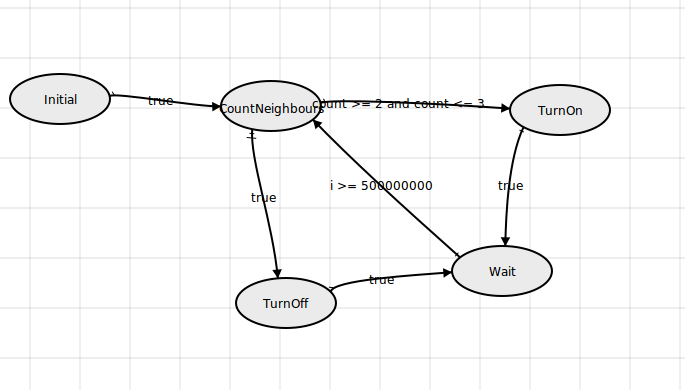
\includegraphics[scale=0.5]{cellularAutomataMachine.png}
		\end{center}
		With variables indicated below:
		\begin{center}
			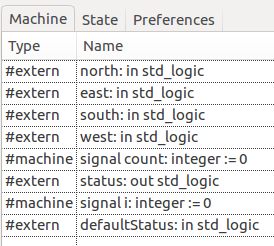
\includegraphics[scale=1]{CellularAutomataMachineVariables.png}
		\end{center}
		The following code will be generated:
		\begin{lstlisting}
			library IEEE;
			use IEEE.std_logic_1164.All;
			
			entity CellularAutomaton is
				port (
					clk: in std_logic;
					EXTERNAL_north: in std_logic;
					EXTERNAL_east: in std_logic;
					EXTERNAL_south: in std_logic;
					EXTERNAL_west: in std_logic;
					EXTERNAL_status: out std_logic;
					EXTERNAL_defaultStatus: in std_logic
				);
			end CellularAutomaton;
			
			architecture LLFSM of CellularAutomaton is
				--Internal State Representation Bits
				constant OnEntry: std_logic_vector(2 downto 0) := "000";
				constant CheckTransition: std_logic_vector(2 downto 0) := "001";
				constant OnExit: std_logic_vector(2 downto 0) := "010";
				constant Internal: std_logic_vector(2 downto 0) := "011";
				constant ReadToSnapshot: std_logic_vector(2 downto 0) := "100";
				constant WriteFromSnapshot: std_logic_vector(2 downto 0) := "101";
				signal internalState: std_logic_vector(2 downto 0) := ReadToSnapshot;
				--State Representation Bits
				constant STATE_Initial: std_logic_vector(2 downto 0) := "000";
				constant STATE_TurnOn: std_logic_vector(2 downto 0) := "001";
				constant STATE_Wait: std_logic_vector(2 downto 0) := "010";
				constant STATE_TurnOff: std_logic_vector(2 downto 0) := "011";
				constant STATE_CountNeighbours: std_logic_vector(2 downto 0) := "100";
				signal currentState: std_logic_vector(2 downto 0) := STATE_Initial;
				signal targetState: std_logic_vector(2 downto 0);
				signal previousRinglet: std_logic_vector(2 downto 0);
				--Snapshot of External Variables
				signal north: std_logic;
				signal east: std_logic;
				signal south: std_logic;
				signal west: std_logic;
				signal status: std_logic;
				signal defaultStatus: std_logic;
				--Machine Variables
				signal count: integer := 0;
				signal i: integer := 0;
				
			begin
			...
		\end{lstlisting}
		On the falling edge of the clock (before the first sub-state in the ringlet), all input snapshot variables will be read from the external variables. The code for the cellular automaton example is seen below:
		\begin{lstlisting}
           when ReadToSnapshot =>
	           north <= EXTERNAL_north;
	           east <= EXTERNAL_east;
	           south <= EXTERNAL_south;
	           west <= EXTERNAL_west;
	           defaultStatus <= EXTERNAL_defaultStatus;
	           if (previousRinglet = currentState) then
		           internalState <= Internal;
	           else
		           internalState <= OnEntry;
	           end if;
		\end{lstlisting}
		At the end of the ringlet and on the rising edge of the clock, the output snapshot variables will be written to the external variables:
		\begin{lstlisting}
			when WriteFromSnapshot =>
				EXTERNAL_status <= status;
				internalState <= ReadToSnapshot;
				if (currentState = targetState) then
					previousRinglet <= currentState;
				else
					currentState <= targetState;
				end if;
		\end{lstlisting}
	\section{Cellular Automata}
		The example used in this document has been the cellular automaton that I've been working on. It should be noted that this example is still not functioning correctly and it would be better to discuss the problems with this at our next meeting.
	\pagebreak
	\section{Appendix}
		The full code for the cellular automaton can be seen below:
		\begin{lstlisting}
			library IEEE;
			use IEEE.std_logic_1164.All;
			
			entity CellularAutomaton is
				port (
					clk: in std_logic;
					EXTERNAL_north: in std_logic;
					EXTERNAL_east: in std_logic;
					EXTERNAL_south: in std_logic;
					EXTERNAL_west: in std_logic;
					EXTERNAL_status: out std_logic;
					EXTERNAL_defaultStatus: in std_logic
				);
			end CellularAutomaton;
			
			architecture LLFSM of CellularAutomaton is
				--Internal State Representation Bits
				constant OnEntry: std_logic_vector(2 downto 0) := "000";
				constant CheckTransition: std_logic_vector(2 downto 0) := "001";
				constant OnExit: std_logic_vector(2 downto 0) := "010";
				constant Internal: std_logic_vector(2 downto 0) := "011";
				constant ReadToSnapshot: std_logic_vector(2 downto 0) := "100";
				constant WriteFromSnapshot: std_logic_vector(2 downto 0) := "101";
				signal internalState: std_logic_vector(2 downto 0) := ReadToSnapshot;
				--State Representation Bits
				constant STATE_Initial: std_logic_vector(2 downto 0) := "000";
				constant STATE_TurnOn: std_logic_vector(2 downto 0) := "001";
				constant STATE_Wait: std_logic_vector(2 downto 0) := "010";
				constant STATE_TurnOff: std_logic_vector(2 downto 0) := "011";
				constant STATE_CountNeighbours: std_logic_vector(2 downto 0) := "100";
				signal currentState: std_logic_vector(2 downto 0) := STATE_Initial;
				signal targetState: std_logic_vector(2 downto 0);
				signal previousRinglet: std_logic_vector(2 downto 0);
				--Snapshot of External Variables
				signal north: std_logic;
				signal east: std_logic;
				signal south: std_logic;
				signal west: std_logic;
				signal status: std_logic;
				signal defaultStatus: std_logic;
				--Machine Variables
				signal count: integer := 0;
				signal i: integer := 0;
			begin
			process (clk)
				begin
					if (rising_edge(clk)) then
						case currentState is
							when STATE_Initial =>
								case internalState is
									when OnEntry =>
										status <= defaultStatus;
										internalState <= CheckTransition;
									when Internal =>
										internalState <= CheckTransition;
									when OnExit =>
										internalState <= WriteFromSnapshot;
										previousRinglet <= currentState;
									when WriteFromSnapshot =>
										EXTERNAL_status <= status;
										internalState <= ReadToSnapshot;
										if (currentState = targetState) then
											previousRinglet <= currentState;
										else
											currentState <= targetState;
										end if;
									when others =>
										null;
								end case;
							when STATE_TurnOn =>
								case internalState is
									when OnEntry =>
										status <= '1';
										internalState <= CheckTransition;
									when Internal =>
										internalState <= CheckTransition;
									when OnExit =>
										internalState <= WriteFromSnapshot;
										previousRinglet <= currentState;
									when WriteFromSnapshot =>
										EXTERNAL_status <= status;
										internalState <= ReadToSnapshot;
										if (currentState = targetState) then
											previousRinglet <= currentState;
										else
											currentState <= targetState;
										end if;
									when others =>
										null;
								end case;
							when STATE_Wait =>
								case internalState is
									when OnEntry =>
										i <= 0;
										internalState <= CheckTransition;
									when Internal =>
										i <= i + 1;
										internalState <= CheckTransition;
									when OnExit =>
										internalState <= WriteFromSnapshot;
										previousRinglet <= currentState;
									when WriteFromSnapshot =>
										EXTERNAL_status <= status;
										internalState <= ReadToSnapshot;
										if (currentState = targetState) then
											previousRinglet <= currentState;
										else
											currentState <= targetState;
										end if;
									when others =>
										null;
								end case;
							when STATE_TurnOff =>
								case internalState is
									when OnEntry =>
									status <= '0';
										internalState <= CheckTransition;
									when Internal =>
										internalState <= CheckTransition;
									when OnExit =>
										internalState <= WriteFromSnapshot;
										previousRinglet <= currentState;
									when WriteFromSnapshot =>
										EXTERNAL_status <= status;
										internalState <= ReadToSnapshot;
										if (currentState = targetState) then
											previousRinglet <= currentState;
										else
											currentState <= targetState;
										end if;
									when others =>
										null;
								end case;
							when STATE_CountNeighbours =>
								case internalState is
									when OnEntry =>
										count <= 0;
										if (north = '1') then
											count <= count + 1;
										end if;
										if (east = '1') then
											count <= count + 1;
										end if;
										if (south = '1') then
											count <= count + 1;
										end if;
										if (west = '1') then
											count <= count + 1;
										end if;
										internalState <= CheckTransition;
									when Internal =>
										internalState <= CheckTransition;
									when OnExit =>
										internalState <= WriteFromSnapshot;
										previousRinglet <= currentState;
									when WriteFromSnapshot =>
										EXTERNAL_status <= status;
										internalState <= ReadToSnapshot;
										if (currentState = targetState) then
											previousRinglet <= currentState;
										else
											currentState <= targetState;
										end if;
									when others =>
										null;
								end case;
							when others =>
								null;
						end case;
					end if;
					if (falling_edge(clk)) then
						case internalState is
							when CheckTransition =>
								case currentState is
									when STATE_Initial =>
										if (true) then
											targetState <= STATE_CountNeighbours;
											internalState <= OnExit;
										else
											internalState <= WriteFromSnapshot;
										end if;
									when STATE_TurnOn =>
										if (true) then
											targetState <= STATE_Wait;
											internalState <= OnExit;
										else
											internalState <= WriteFromSnapshot;
										end if;
									when STATE_Wait =>
										if (i >= 500000000) then
											targetState <= STATE_CountNeighbours;
											internalState <= OnExit;
										else
											internalState <= WriteFromSnapshot;
										end if;
									when STATE_TurnOff =>
										if (true) then
											targetState <= STATE_Wait;
											internalState <= OnExit;
										else
											internalState <= WriteFromSnapshot;
										end if;
									when STATE_CountNeighbours =>
										if (count >= 2 and count <= 3) then
											targetState <= STATE_TurnOn;
											internalState <= OnExit;
										elsif (true) and (not (count >= 2 and count <= 3)) then
											targetState <= STATE_TurnOff;
											internalState <= OnExit;
										else
											internalState <= WriteFromSnapshot;
										end if;
									when others =>
										null;
								end case;
							when ReadToSnapshot =>
								north <= EXTERNAL_north;
								east <= EXTERNAL_east;
								south <= EXTERNAL_south;
								west <= EXTERNAL_west;
								defaultStatus <= EXTERNAL_defaultStatus;
								if (previousRinglet = currentState) then
									internalState <= Internal;
								else
									internalState <= OnEntry;
								end if;
							when others =>
								null;
						end case;
					end if;
			end process;
			end LLFSM;
		\end{lstlisting}
\end{document}